\documentclass[sigconf]{acmart}

\usepackage{booktabs} % For formal tables
% packages & styles
\usepackage{comment}
\usepackage{graphicx}     % Insert figures
\usepackage{setspace}      % line distance
\usepackage{bbding}        % yes and no
\usepackage{amssymb, amsmath}    % American Math Society, Symbols, Math equations
\usepackage{pifont}         % Add a circle around 'x' (\textcircled{x})
\usepackage{times}          % Times New Roman
%\usepackage{booktabs}    % Tables, http://ddswhu.com/2014/08/24/9-essential-latex-packages/
\usepackage{multicol, multirow}     % Double collumns, rows
\usepackage{float}           % Figure Positions
\usepackage{makecell}    % Table Cell
%\usepackage{url}              % Add url in the references, http://blog.csdn.net/perfumekristy/article/details/8680045
\usepackage{threeparttable} % Three part table
%\usepackage{subfigure}   % Insert 2 figures side by side
\usepackage{algorithm,algpseudocode}    % Pseudo code
\usepackage{lettrine}       % A large letter at the fisrt letter of the article.
%\usepackage{mathrsfs}    % Bold curlycue - cause error in ACM 2017 template (MAC)
%\usepackage{vector}       % Arrow on the letters: vector
%\usepackage[nocompress]{cite}   % Citation: [1,2,3,4]
%\usepackage{cite}           % Citation: [1-4]
%\usepackage[numbers,sort&compress]{natbib}
\usepackage[colorlinks, linkcolor=default, anchorcolor=default, citecolor=default]{hyperref} % generate a content index in PDF

\graphicspath{{images/}}

%##############################################################################
% Fonts
%##############################################################################
%\begin{comment}
\newcommand{\Fsize}[2][.]{%
    \ifthenelse{\equal{#1}{.}}{
        \fontsize{#2}{#2}%
    }{%
        \fontsize{#2}{#1}%
    }%
    \selectfont%
}


%##############################################################################
% Tables
%##############################################################################
%\begin{comment}
\newcommand{\Drop}[1]{%
    \multirow{2}{*}{#1}%
}
\newcolumntype{I}{!{\vrule width 0.8pt}}
\newenvironment{newitemize}{
    \begin{itemize}
      \setlength{\itemsep}{0pt}
      \setlength{\parskip}{0pt}
      \setlength{\parsep}{0pt}
}{\end{itemize}}
\setlength{\intextsep}{5pt plus 3pt minus 3pt}
%\setlength\textfloatsep{1.25\baselineskip plus 1pt minus 1pt}
%\end{comment}
%##############################################################################
% Algo
%##############################################################################
%\RestyleAlgo{ruled}

%\renewcommand{\algorithmicrequire}{\textbf{Input:}} % Use Input in the format of Algorithm
%\renewcommand{\algorithmicensure}{\textbf{Output:}} % Use Output in the format of Algorithm 


% Copyright
\setcopyright{none}
%\setcopyright{acmcopyright}
%\setcopyright{acmlicensed}
%\setcopyright{rightsretained}
%\setcopyright{usgov}
%\setcopyright{usgovmixed}
%\setcopyright{cagov}
%\setcopyright{cagovmixed}

% DOI
\acmDOI{}

% ISBN
\acmISBN{}

%Conference
\acmConference[DAC'2018]{}{May 2018}{San Francisco, CA, US} 
\acmYear{}
\copyrightyear{}


\acmArticle{}
\acmPrice{}

\begin{document}
\title{An Energy Behavior Supporting Simulator for Nonvolatile Processor Based Self-powered System.}

\begin{comment}
\titlenote{Produces the permission block, and
  copyright information}
\subtitle{Extended Abstract}
\subtitlenote{The full version of the author's guide is available as
  \texttt{acmart.pdf} document}
\end{comment}

\begin{comment}
\author{Ben Trovato}
\authornote{Dr.~Trovato insisted his name be first.}
\orcid{1234-5678-9012}
\affiliation{%
  \institution{Institute for Clarity in Documentation}
  \streetaddress{P.O. Box 1212}
  \city{Dublin} 
  \state{Ohio} 
  \postcode{43017-6221}
}
\email{trovato@corporation.com}
\end{comment}

% The default list of authors is too long for headers.
%\renewcommand{\shortauthors}{B. Trovato et al.}

% As a general rule, do not put math, special symbols or citations
% in the abstract
% As a general rule, do not put math, special symbols or citations
% in the abstract
\begin{abstract}
%
Battery-less devices and energy harvesting techniques are more and more attractive in today's IoT area. However, the intermittent and low-intensity ambient power sources cause insecure quality of service (QoS) of these self-powered IoT applications, which makes it essential to pre-simulate the QoS of an self-powered system and its energy managing strategy under various power conditions. Unfortunately, existing simulator lacks of supports on peripherals in a self-powered system and requires great efforts to implement the hardware-based energy managing schemes, such as NVP, DVFS and near-threshold designs. 

This paper proposes EBeSS, an system-level simulator based on GEM5, supporting easy-configurable energy managing strategies on both processor and peripherals. EBeSS develops a configurable simulation object, virtual device, to support the functional and energy-related behaviors of peripherals, and energy message handling framework to support configured energy managing strategies. A real hardware prototype validates that the error of EBeSS is less that xx\%. And a self-powered system design flow is given to reveal the potential of EBeSS on exploring the design space of parameters of a self-powered system (such as capacitor and energy managing scheme) with optimal performance.

\end{abstract}

% no keywords

\maketitle

\section{Introduction}	\label{sec:intro}
%
Battery-less devices are more and more popular in today's IoT area for its light-weight charge-free energy supply system and long lifetime.
However, the energy supply quality of these devices is insecure according to different energy sources and different working environment.
For instance, solar-power is the most popular ambient energy source, whose power supply intensity various within orders of micro-watt to milliwatt according to the time, season, weather condition, altitude, location (indoor/outdoor) and etc. 
Therefore, developers need to evaluate the quality of service (QoS) of a self-powered system under specific power supply condition before developing an energy harvesting application.
Without proper software simulator, developers have to implement a hardware prototype with appropriate energy managing strategies to realize evaluate quality of service (QoS), which costs unacceptable efforts and time.

%
To tackle this problem, previous works develop different simulation strategies for different types of self-powered devices.
Target the systems with pure software energy managing and scheduling algorithms, EDB~\cite{Colin2016An} proposes an energy supporting debugger to simulate the performance of intermittent powered devices.
For the devices with hardware optimizations, such nonvolatile processor (NVP)~\cite{wang20123us,wang2017a,Su2016A,Liu2015Ambient}, NVIO~\cite{li2016hw}, NVRF~\cite{wang2017a130nm}, and near-threshold circuits~\cite{}, Ma et al.~\cite{Ma2015Architecture} provides a simulating strategy based on verilog source code to process register-transfer level (RTL) evaluation.
Furthermore, Gu et al.~\cite{gu2016nvpsim} models the architecture and energy managing behaviors of NVP~\cite{wang20123us} and proposes NVPsim, a simulator based on GEM5 to explore the processor-level parameter design space of NVP.

%
Although provided usable simulation approaches for processor and software energy managing algorithms, the above mentioned simulation tools has two main draw backs. 
Firstly, these simulators cannot support the functional and energy-related behaviors of peripherals.
Peripherals, such as sensors, radio transceivers and accelerators, are playing irreplaceable roles in IoT area by taking charge of the interconnections between the system and the environment, and improve the QoS. 
With intermittent power supply, these external hardware modules may cause inconsistency problems and needs to be safely recovered after sudden outages.
Secondly, neither RTL-level simulation~\cite{Ma2015Architecture} nor NVPsim~\cite{gu2016nvpsim} supports flexible and easy configured hardware energy managing techniques such as NVP~\cite{wang20123us} and dynamic voltage-frequency scaling (DVFS)~\cite{}.

%
Focus on these problems, this paper proposes EBeSS, an \underline{\textbf{E}}nergy \underline{\textbf{Be}}havior \underline{\textbf{S}}upporting \underline{\textbf{S}}ystem-level simulator to explore the design space of a NVP based self-powered device.
%This paper presents the structure of the simulator and executes design space explorations on three existing energy behavior schemes.
The contributions are listed as follows,
\begin{itemize}
	\item Based on GEM5, EBeSS provides a configurable virtual device module to support the simulation of a variety of peripherals; 

     \item EBeSS realizes flexible and friendly hardware energy managing behavior supports with the help of the energy message handling (EMH) framework to realize and manage  the energy-related behaviors of each hardware module; 

	\item With EBeSS, we provides an example of self-powered system developing and optimizing procedure by exploring the design space of capacitor and energy managing strategy selection with different power traces and benchmarks. The analysis reveals an optimal design edge to improve the performance of self-powered systems.
\end{itemize}

The rest of the paper is organized as follows.
Sec.~\ref{sec:tech} proposes the architecture of the simulator and introduces the two techniques used to support the energy behavior exploration of NVP and peripherals.
Sec.~\ref{sec:valid} validates the functionality of EBeSS with a real NVP based self-powered system prototype.
Sec.~\ref{sec:exp} explores the performance of different energy behaviors with various power supply profile and application types.
Finally, Sec.~\ref{sec:sum} summarizes the whole paper and looks ahead for more advanced usages of EBeSS.

\begin{comment}
  \bibliographystyle{ACM-Reference-Format}
  \bibliography{references}
\end{comment}
\section{EBeSS Design Methodology}	\label{sec:tech}
%
This section demonstrates the design methodology of EBeSS.
After introducing the overview of EBeSS structure, we illustrates the two key techniques embedded in the simulator.
\emph{Virtual Device} is a configurable module used to simulate the behaviors of peripherals.
\emph{Energy Message Handling Framework (EMHF)} provides an energy message interacting structure to manage the energy-related behaviors of each hardware module according to the energy managing strategies.

\subsection{Structure Overview of EBeSS}		\label{sec:tech-structure}
%
EBeSS is an GEM5-based system-level simulator for self-powered systems. 
EBeSS adopts the fundamental usage and logic of kernel architecture in GEM5 and develops two novel components to support peripherals and energy management.
EBeSS enables the ability of simulating the energy-related behaviors of self-powered systems, such as non-volatile processors, multi-frequency systems, and multi-voltage-domain systems. 
The system architecture of EBeSS is shown in Figure~\ref{fig:techStructure}.

\begin{figure}[!htpb]
	\centering
	\vspace{-10pt}
	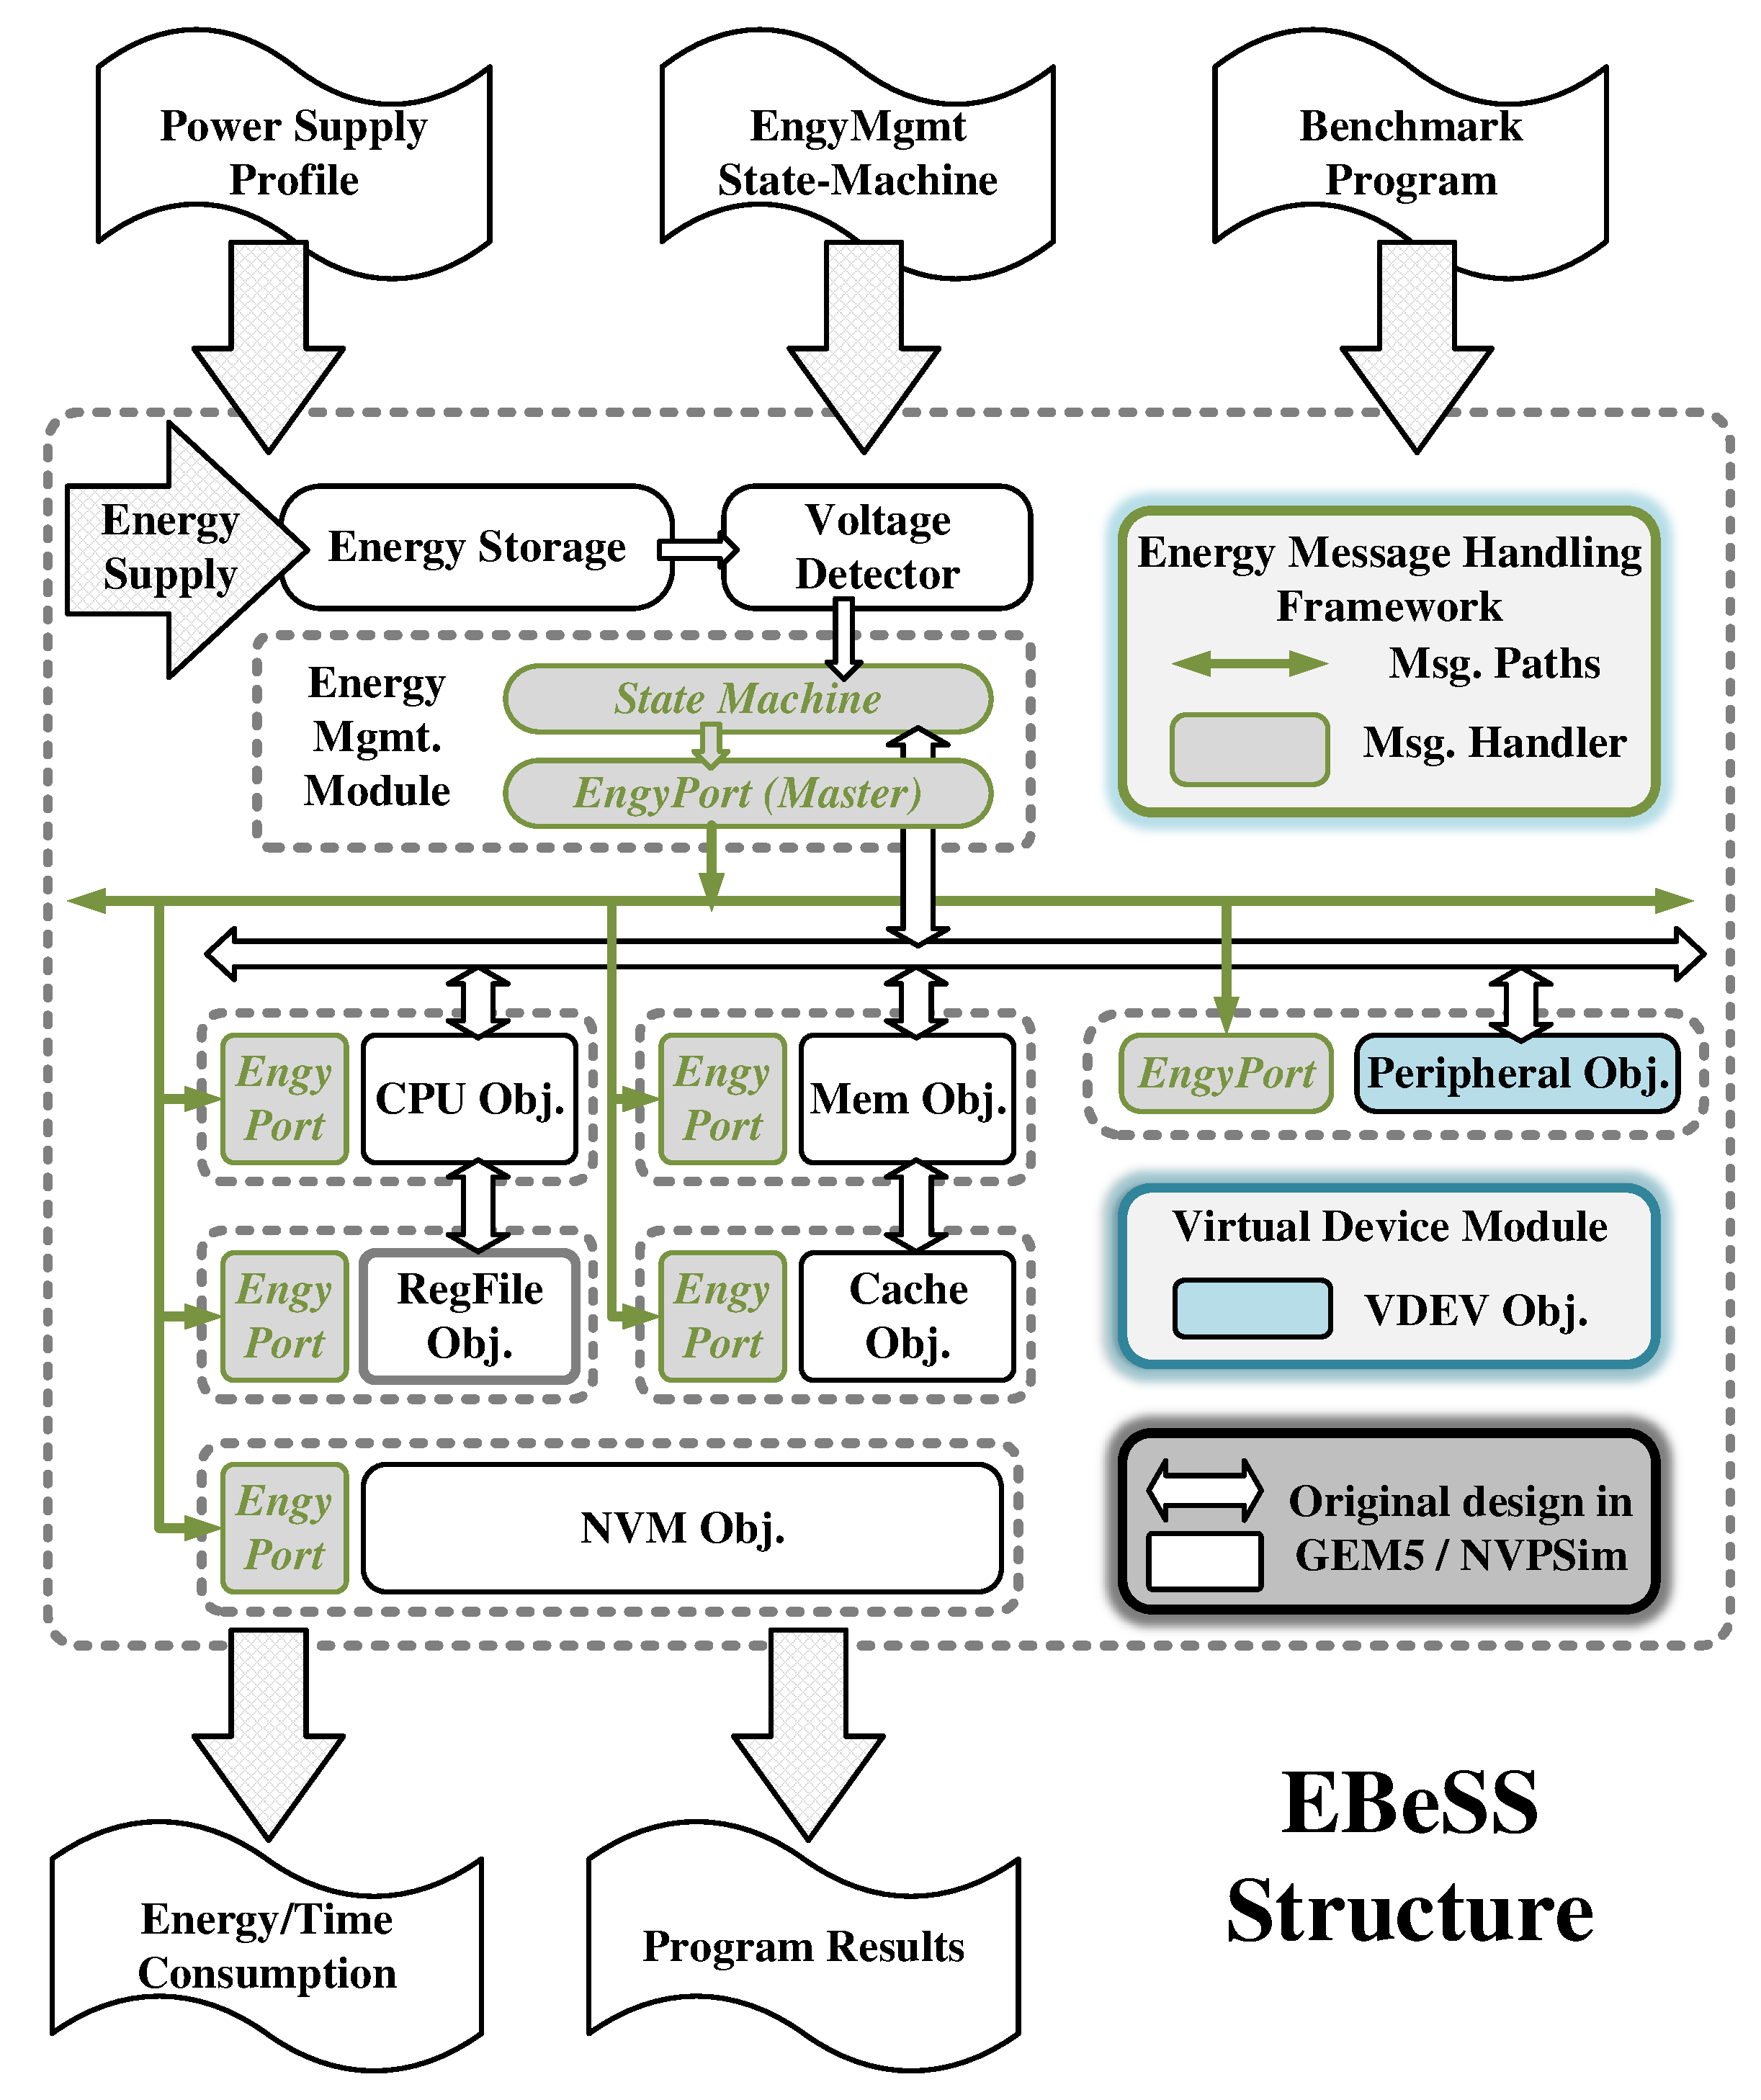
\includegraphics[width=0.5\textwidth]{EBeSS_Structure}
	\vspace{-20pt}
	\caption{Simulator structure of EBeSS. Two new components are added based on original GEM5 architecture. EMHF generates and handles the energy messages according to energy conditions. The virtual device module creates an configurable object that supports the functionary and energy-related behaviors of peripherals.}		\label{fig:techStructure}
\end{figure}

%
To fill the blank of lacking peripheral supports, EBeSS adopts a new simulation object, \emph{virtual device}, which defines the connections and functionary behaviors of various peripherals, as shown in Figure~\ref{fig:techStructure}.
Virtual device is a configurable, pluggable module connected the system bus, which can be accessed by processor module via virtual addresses. 
Virtual device supports the fundamental operations of a peripheral, including the peripheral register read/write, initialization, activation and interrupts.
Details of the virtual device module is discussed in Section~\ref{sec:tech-vdev}.

%
EMHF provides a message-based energy managing framework to support configurable energy managing strategies, as shown in Figure~\ref{fig:techStructure}.
EMHF contains three components, energy management module (EMM), energy ports and energy objects. 
EMM contains a state machine to generate the state conversion according to user's energy managing strategy. 
Energy ports define the energy message transmission rules and manage the interconnections between EMM and other hardware components.
For each hardware component, EMHF reconstructs it with a new energy-related object, energy object (EnergyObject) allowing energy behaviors defined by energy management strategies as a reaction to energy condition changes.
Details of the energy message handling framework is discussed in Section~\ref{sec:tech-EMHF}.


\subsection{Peripheral Support: Virtual Device}	\label{sec:tech-vdev}
%
Although GEM5 provides powerful simulation ability to estimate the functionalities of processor and memories, supports are still vacant for various peripherals, such as sensors and radio transmitter, which play indispensable roles in energy harvesting systems.
To support the peripherals, this subsection first gives a general model of a peripheral and then introduces the proposed hardware component, virtual device.

\textbf{Peripheral Modeling\ \ }
%
Figure~\ref{fig:PeripheralModel} (a) shows the structure model a typical digital peripheral.
The model contains a digital part to realize data storage and control logics, and an analog part to realize specific functionality.
The digital part contains an internal register file to store the command, execution status and data.
The processor can access a peripheral by writing commands to the \emph{cmd\_reg} and read from the \emph{data\_reg}.
When a new command arrives, the changing bits in the \emph{cmd\_reg} will trigger operations, such as initialization, sensing and radio transmission.

Figure~\ref{fig:PeripheralModel} (b) shows a typical peripheral working flow.
A peripheral needs to be initialized to get ready before executing other tasks.
When a task (collecting a data) is completed, the peripheral will trigger an interrupt to inform the processor for subsequence operations.

\begin{figure}[!htpb]
	\centering
	\vspace{-5pt}
	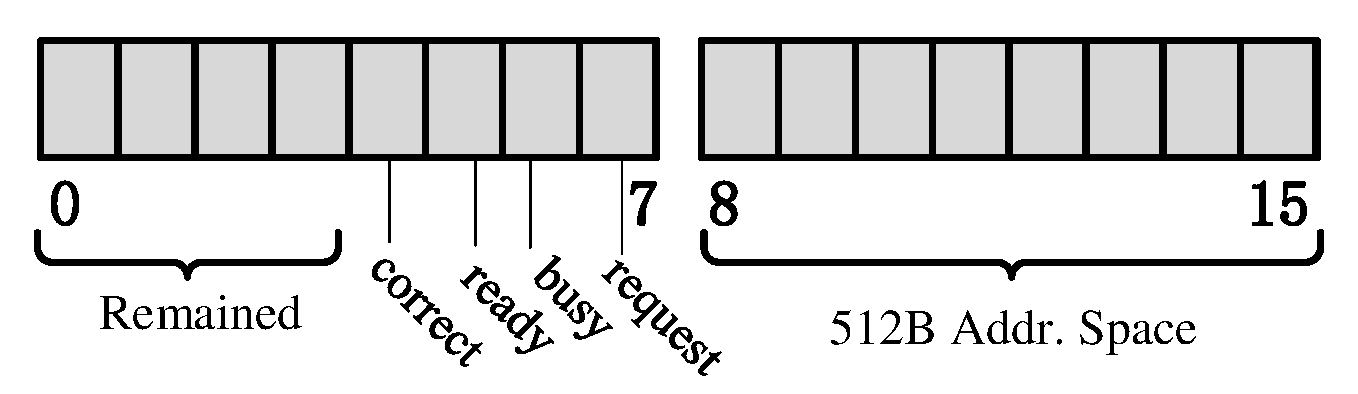
\includegraphics[width=0.4\textwidth]{VirtualDeviceAddress}
	\vspace{-5pt}
	\caption{The structure model (a) and a typical working flow (b) of common digital peripherals.}	\label{fig:PeripheralModel}
\end{figure}

\textbf{Virtual Device Object\ \ }
EBeSS proposes a configurable virtual device object defining the peripheral behaviors and the interconnections between peripherals and the processor, as shown in Figure~\ref{fig:VirtualDevice} (a).
Virtual device is a memory-like module that the processor can make a request by accessing the address of virtual device. 
When the processor accesses a registered virtual address, the system will forward this access to the physical address of the related virtual device.
The address of virtual devices consists of a control byte and a maximum 511B internal memory space bytes as data bytes, as shown in Figure~\ref{fig:VirtualDevice}.
In the control byte, four bits are used to control the executing status of peripherals.
\emph{addr1} is a configurable \emph{init} bit to trigger the initialization operation.
\emph{addr2} is a read-only \emph{ready} bit representing whether a device is initialized.
\emph{addr5} is a read-only \emph{complete} bit and will be set and trigger an interrupt to the processor, when a virtual device operation is finished.
\emph{addr5} is a read-only \emph{busy} bit representing whether the device is during execution and is not accessible if the bit is set.
\emph{addr7} is a configurable bit set by CPU to make a request to a virtual device.

EBeSS requires users to modify peripheral-related programs to suit the design of virtual device.
Figure~\ref{fig:VirtualDevice} (b) shows a program of temperature sensing task. 
Before all, the sensor has to declare its virtual space range and the address of its \emph{cmd\_reg}. 
In energy limited scenarios, energy harvesting system has no operating system to support automatic allocate address spaces for peripheral.
Therefore, EBeSS allows virtual devices to register virtual addresses.
Then, the initialization command is load to the \emph{cmd\_reg} to prepare the sensor.
After the sensor state is ready, the system activates the sensor to start a sensing tasks.
When the sensing task is completed, the processor checks the \emph{complete} state bit and fetch the collected data from \emph{data\_reg}.

\begin{figure}[!htpb]
	\centering
	\vspace{-5pt}
	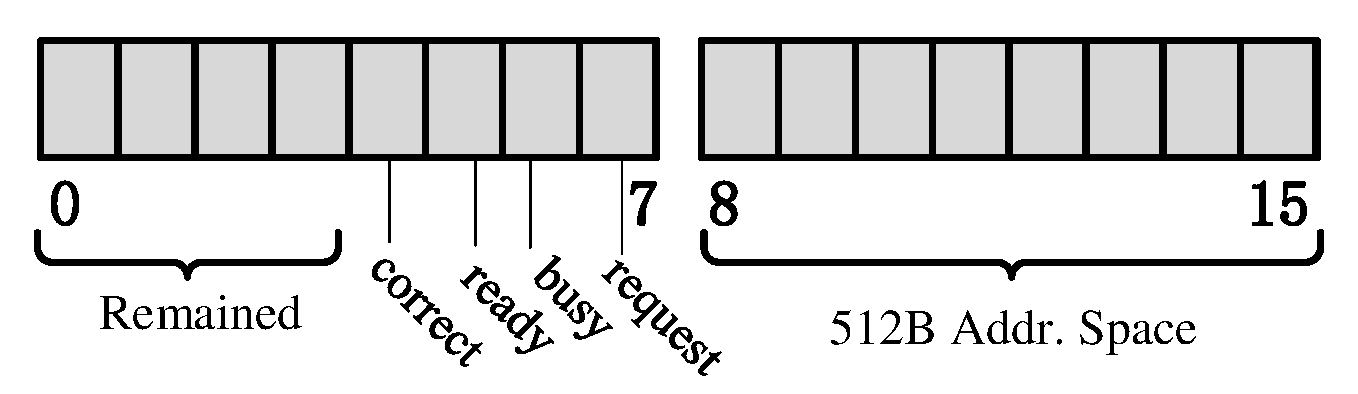
\includegraphics[width=0.4\textwidth]{VirtualDeviceAddress}
	\vspace{-5pt}
	\caption{The bit-level explanation of virtual device address definition.}	\label{fig:VirtualDevice}
\end{figure}

\subsection{Energy Message Handling Framework (EMHF)}	\label{sec:tech-EMHF}
% Overview
EMHF is a message-based event handling framework to support the energy managing strategies in a self-powered system.
The framework consists of three components: the informer, the connector and the reactor, as shown in Figure~\ref{fig:EngyMsgFrameworkStructure}. 
With these components, EMHF realize the functionality of energy harvesting, monitoring and all the detailed energy-related behaviors of each hardware component according to energy managing strategies.

\begin{figure}[!htpb]
	\centering
	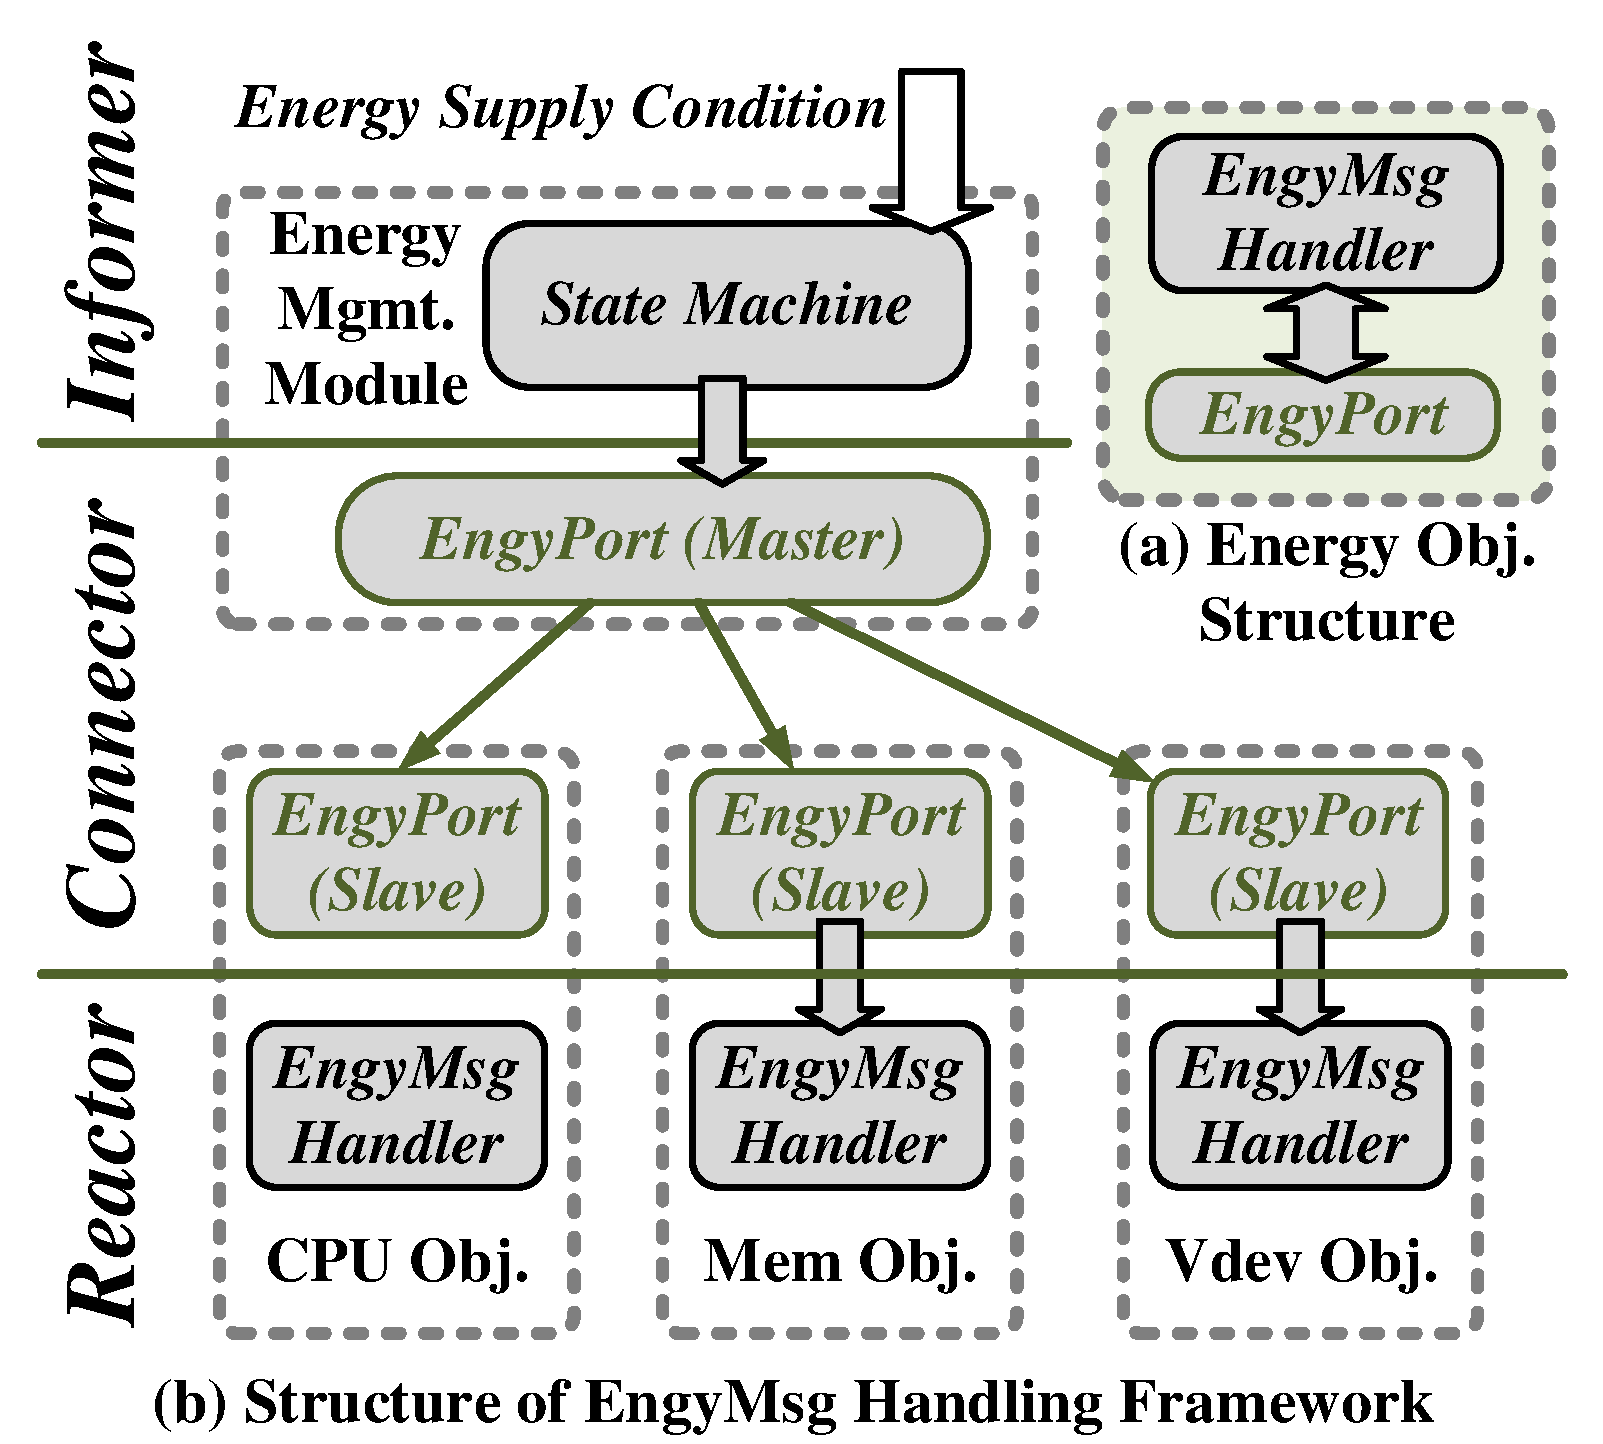
\includegraphics[width=0.45\textwidth]{EngyMsgFrameworkStructure}
	\vspace{-5pt}
	\caption{Structure of the energy message handling framework. The framework contains three components, the informer, the connector and the reactor.}		\label{fig:EngyMsgFrameworkStructure}
	%\vspace{-15pt}
\end{figure}

\textbf{Informer: Energy Management Module.\ \ }
% EMM
In the energy message handling framework, an energy management module (EMM) is developed to monitor energy changes and broadcast state conversion messages according to a user-defined energy managing strategy.
EMM consists of a energy storage, a harvester, a consumer and a state machine, as shown in Figure~\ref{fig:EnergyManagementModule}. 
During each time tick, the energy harvester collects the income energy from an energy profile and consumer will collect energy consumptions from all the other hardware modules. 
These energy changes are committed to the energy storage (capacitors). 
The state machine is configurable to realize and explore the optimal design of the user-defined energy managing strategies. 
When the supply voltage in the storage reaches certain thresholds, EMM determines state conversion messages according to the state machine and broadcast to the entire system.

\begin{figure}[!htpb]
	\centering
	\vspace{-5pt}
	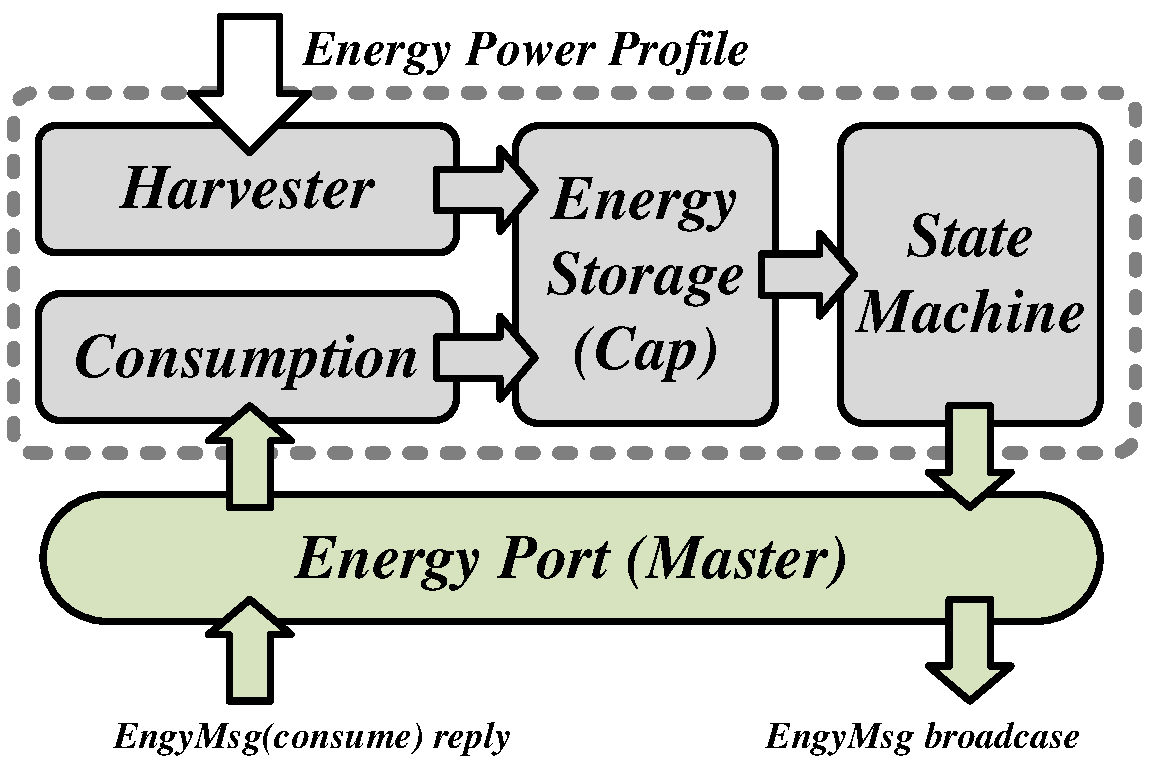
\includegraphics[width=0.35\textwidth]{EnergyManagementModule}
	\vspace{-10pt}
	\caption{The structure and work flow of the energy management module.}		\label{fig:EnergyManagementModule}
\end{figure}

\textbf{Reactor: Energy Object.\ \ }
% Energy Reactor
Except for EMM, all the other hardware modules are defined as reactors, including the processor, memory and virtual devices.
In GEM5, the native simulation object for these module supports only the functionary behaviors such as computing and memory accessing operations.
To support the energy-related behaviors, EBeSS extend an energy object for each hardware module.
An energy object contain an energy message handler, an consumer and is connected to in EMHF framework via energy ports (introduced later), as shown in Figure~\ref{fig:EngyMsgFrameworkStructure} (b). 
The energy message handler is a programmable module to realize the detailed reactions defined in an energy managing strategy.
According to developers' needs, the handler will adjust the run-time states and parameters, such as reaction delay, consumption, frequency and register data, to reply the upcoming energy messages.
The consumer is used to manage all the run-time energy consumptions, including execution consumption and leakages.
Every tick or after a message reaction, the consumer should reply its energy consumption in a specific energy consuming message format to EMM to commit the energy costs.
In future, EBeSS will open more authorities that the reactor replying more kinds of energy messages under the premise of system robustness.

\textbf{Connector: Energy Ports.\ \ }
% Energy Port
Energy Ports are interfaces that construct connections and exchange energy messages within EMM and energy objects. 
There are two types of energy ports: master port and slave port.
Master ports are connected to multiple slave ports and maintain a list of its slaves during simulation.
In EBeSS, master port is adopted in EMM module as global energy message informer to actively broadcast energy messages in the entire system.
Slave ports are can only track its unique master.
In EBeSS, all the reactors (hardware modules) are connected to slave ports which is used to receive upcoming energy message and reply consumptions.
Note that, master ports can only connect to slave ports, and vice versa.
All the connections are established by users determining master for each slave port in the configuration profile. 
Currently, only one master port is alternative in EBeSS, hence, all the slave ports have to be connected to EMM.

\begin{comment}
\bibliographystyle{ACM-Reference-Format}
\bibliography{references} 
\end{comment}
\section{Simulator Validation}	\label{sec:valid}
%
To validate the correctness and accuracy of EBeSS, we compare the execution parameters of EBeSS with a real NVP-based system prototype~\cite{wang2017a130nm} as shown in Figure~\ref{fig:HardwarePrototype}.
A bridge monitoring application and several independent tasks are executed to compare the performance and energy parameters.

% hardware parameters
\subsection{System configurations}
The configuration of the system prototype is listed in Table~\ref{}. 
This prototype is an solar-powered system, which contains a nonvolatile processor (NVP)~\cite{wang20123us,Liu2015Ambient}, a nonvolatile radio transmitter (NVRF)~\cite{wang2017a130nm} and several volatile sensors.

\begin{figure}[!htpb]
	\centering
	\vspace{-5pt}
	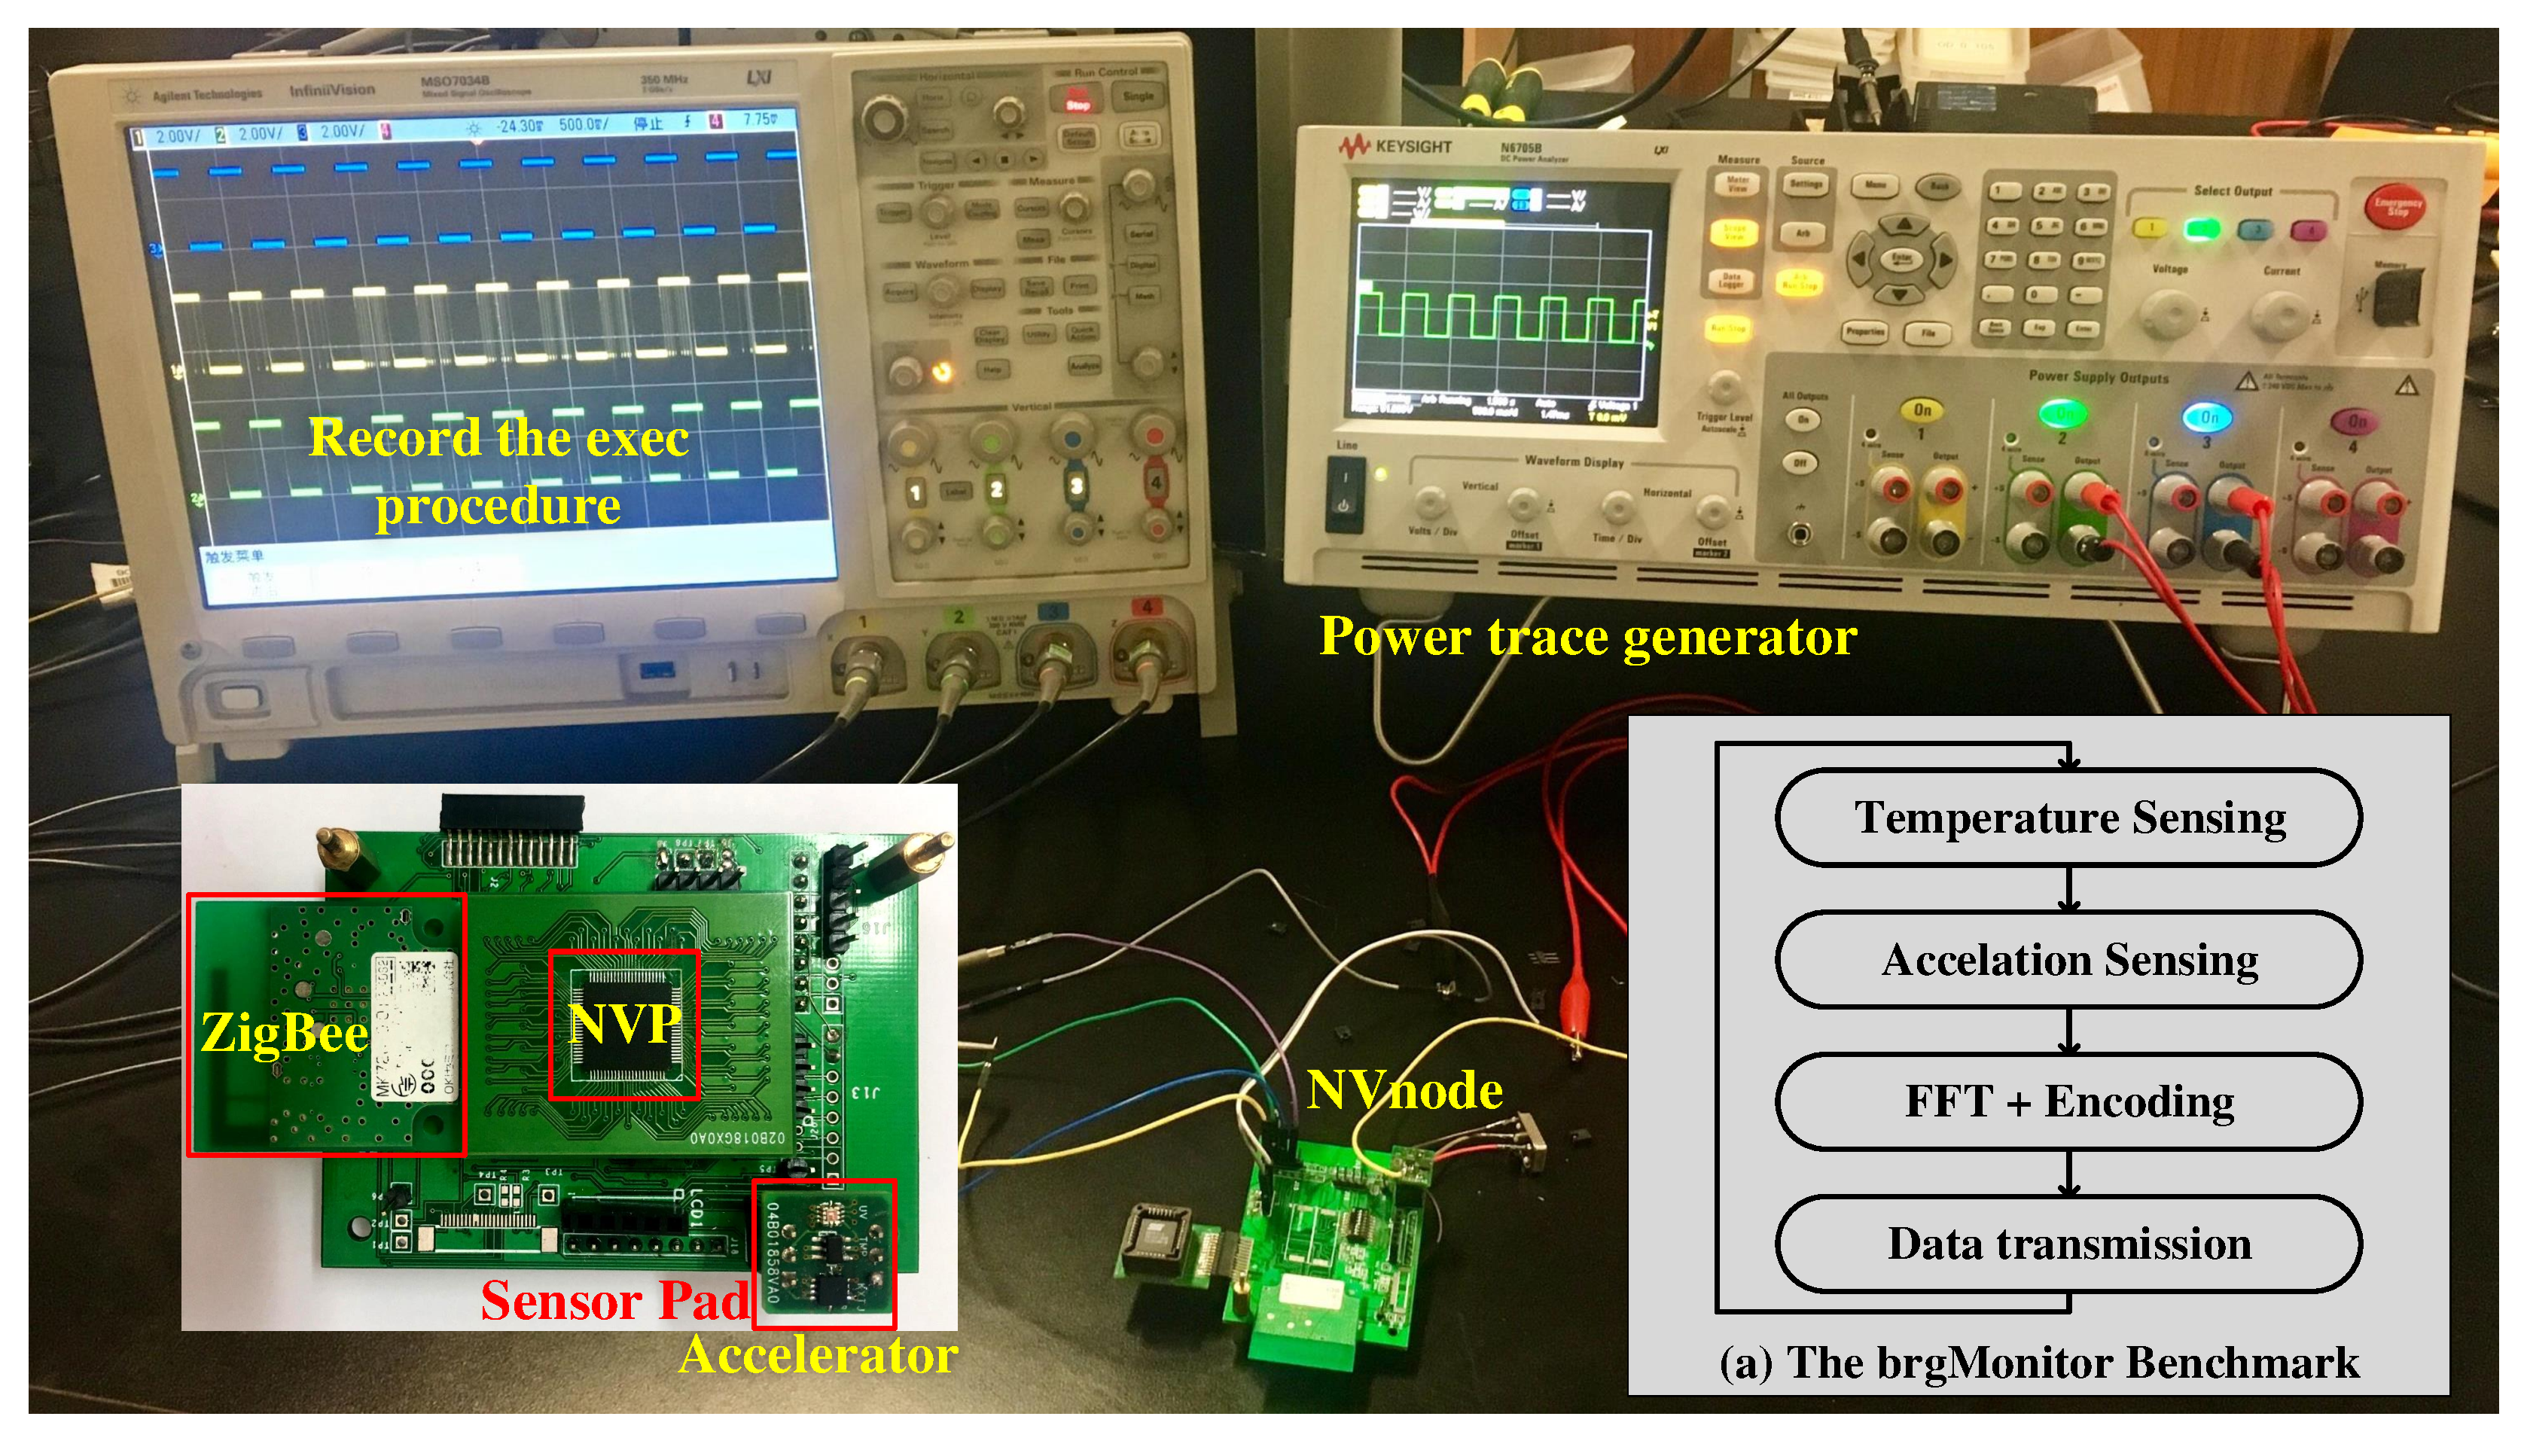
\includegraphics[width=0.48\textwidth]{HardwarePrototype}
	\vspace{-5pt}
	\caption{The hardware prototype used to validate EBeSS simulator. A real bridge monitoring benchmark is utilized to validate the simulator.}	\label{fig:HardwarePrototype}
\end{figure}

NVP enables a two-threshold backup/restore energy managing strategy (\emph{2-thr})~\cite{wang20123us,gu2016nvpsim}, where a lower threshold $V_{low}$ and a higher threshold $V_{high}$ are defined.
When the supply voltage falls below $V_{low}$, the processor immediately backup the execution status to NVM with the help of a control circuit.
When the supply voltage raises above $V_{high}$, the processor restarts and restores all the states and keep on progress.

NVRF is a nonvolatile interface that can automatically recover the radio transmitter and retransmit the uncompleted packet transmission after outages.
Inheriting the two voltage thresholds in \emph{2-thr}, NVRF can backup the configurations of the radio transmitter when the voltage is lower than $V_{low}$, and will reinitialize the transmitter states, resume the configurations and restart the uncompleted transmission.

In addition, the prototype also contains a thermometer and an accelerometer. 
The capacitor is $15uF$. 
All the above hardware parameters are listed in Table~\ref{}.
The power profiles are solar power traces from MIDC database of NREL Solar Radiation Research Laboratory~\cite{midc2015solar}.

% hardware parameters
\subsection{Application Validation}
We compare the simulation result with the hardware execution result using a real IoT application, bridge monitoring application (\emph{brgMonitor}).
The work flow of \emph{brgMonitor} is shown in Figure~\ref{fig:BrgMonitor}.
The device executes a 'sense-process-transmit' cycle to collect bridge health related parameters.
The execution time and energy consumption comparison is shown in Table~\ref{}.
% The error is ...

\begin{figure}[!htpb]
	\centering
	\vspace{-5pt}
	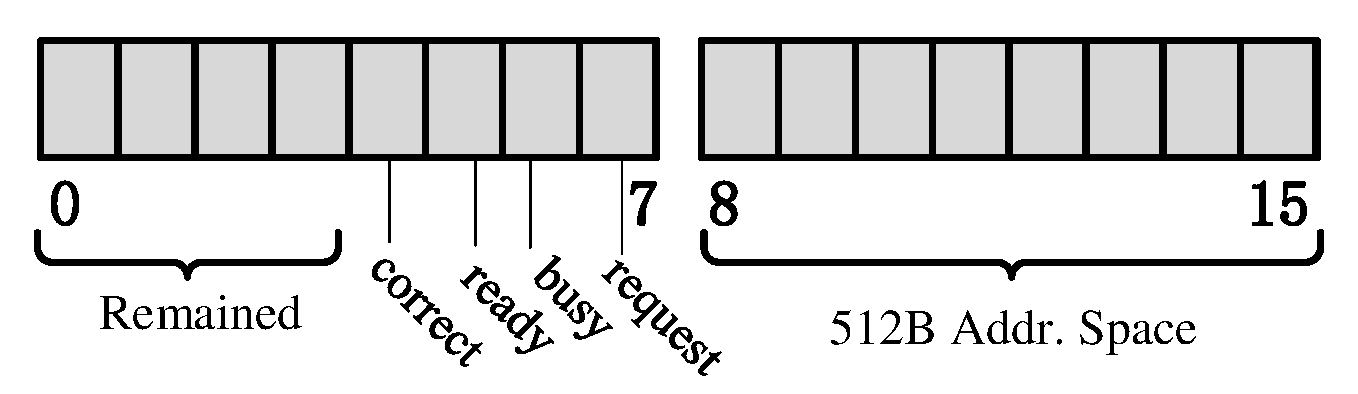
\includegraphics[width=0.4\textwidth]{VirtualDeviceAddress}
	\vspace{-5pt}
	\caption{The working flow and parameters of \emph{brgMonitor} benchmark.}	\label{fig:BrgMonitor}
\end{figure}

Furthermore, we also evaluate the correctness of EBeSS with multiple small tasks in Table~\ref{}.
The maximum error is limited within XXX.

%\begin{table}[t]
	\begin{center}
		%\vspace{-0pt}
		\caption{Parameter Settings of NVP System Prototype~\cite{Liu2015Ambient}.} \label{tab:valid-param}
		%\vspace{-5pt}
		\Fsize{8}
		\renewcommand{\arraystretch}{1.5}
		%\setlength{\tabcolsep}{1pt}
		\begin{tabular}{Ic|c|c|c|c|cI}
			\Xhline{1.2pt}
			Param.	& Oper. Freq.	& power	& Mem	& RegFile	& Cap.\\
			\Xhline{1pt}
			Value	& $1$MHz	& $0.16$mW	& $512$KB	& $128$B	& $10\mu F$\\
			\Xhline{1.2pt}
		\end{tabular}
		\vspace{-15pt}
	\end{center}
\end{table} 
%\begin{table}[t]
	\begin{center}
	\caption{Comparison Between EBeSS and NVP Prototype.} \label{tab:valid-result}
	\vspace{-10pt}
	\Fsize{8}
	\renewcommand{\arraystretch}{1.5}
	\setlength{\tabcolsep}{1.8pt}
	\begin{tabular}{Ic|cIc|c|cIc|c|cIc|c|cI}
		\Xhline{1.2pt}
		\multicolumn{2}{IcI}{}	& \multicolumn{3}{cI}{FFT}		& \multicolumn{3}{cI}{QUEENS}	& \multicolumn{3}{cI}{SORT} \\
		\Xhline{1.2pt}

		Power	& Metrics		& Sim.	& Mea.	& Err.			& Sim.	& Mea.	& Err.			& Sim.	& Mea.	& Err. \\

		\Xhline{1pt}
		\multirow{2}[1.2]{*}{Trace 1}
			& engy./uJ		& 4.21	& 4.02	& 4.51\%		& 7.61	& 7.45	& 2.10\%		& 29.2	& 26.9	& 7.88\% \\
		\cline{2-11}
			& time/ms		& 39.2	& 36.7	& 6.38\%		& 77.4	& 74.3	& 4.01\%		& 266	& 253	& 4.89\% \\

		\Xhline{1pt}
		\multirow{2}[1.2]{*}{Trace 2}
			& engy./uJ		& 2.98	& 2.93	& 1.68\%		& 5.14	& 4.97	& 3.31\%		& 16.2	& 15.4	& 4.94\% \\
		\cline{2-11}
			& time/ms		& 21.2	& 20.6	& 2.83\%		& 51.1	& 49.6	& 2.94\%		& 172	& 166	& 3.49\% \\

		\Xhline{1pt}
		\multirow{2}[1.2]{*}{Trace 3}
			& engy./uJ		& 2.19	& 2.15	& 1.83\%		& 2.97	& 2.91	& 2.02\%		& 10.9	& 10.6	& 2.75\% \\
		\cline{2-11}
			& time/ms		& 14.5	& 14.4	& 0.69\%		& 24.5	& 24.5	& 0.00\%		& 91.1	& 90.2	& 0.99\% \\

		\Xhline{1.2pt}
	\end{tabular}
	\end{center}
	\vspace{-20pt}
\end{table} 

\begin{comment}
\bibliographystyle{ACM-Reference-Format}
\bibliography{references} 
\end{comment}
\section{Design Space Exploration on EBeSS}	\label{sec:exp}
%
EBeSS is an energy-aware simulator supporting peripheral and energy managing strategy configurations for self-powered system.
With EBeSS, developers can optimize the hardware parameters of self-powered system (such as the capacitor size), and select appropriate energy managing strategy to achieve the maximum task completion performance. 
This section explores the design space of capacitor and energy managing strategy selection under different power traces and different peripheral numbers.

\subsection{Capacitor Design Space Considering Peripherals}
%
In this part, we explore the capacitor design space for self-powered system with different number of peripherals. 
Based on the \emph{brgMonitor} application, we scale the peripheral number in the application from zero to five, and simulate the completed task number within 10 minutes.
Figure~\ref{fig:CapVsBenchmark} shows the design space of capacitor size in self-powered system.
% Explainations.
From the figure, we observe a design edge for a self-powered system with different occupancy of peripherals to optimize the task completion rate.

\begin{figure}[!htpb]
	\centering
	\vspace{-5pt}
	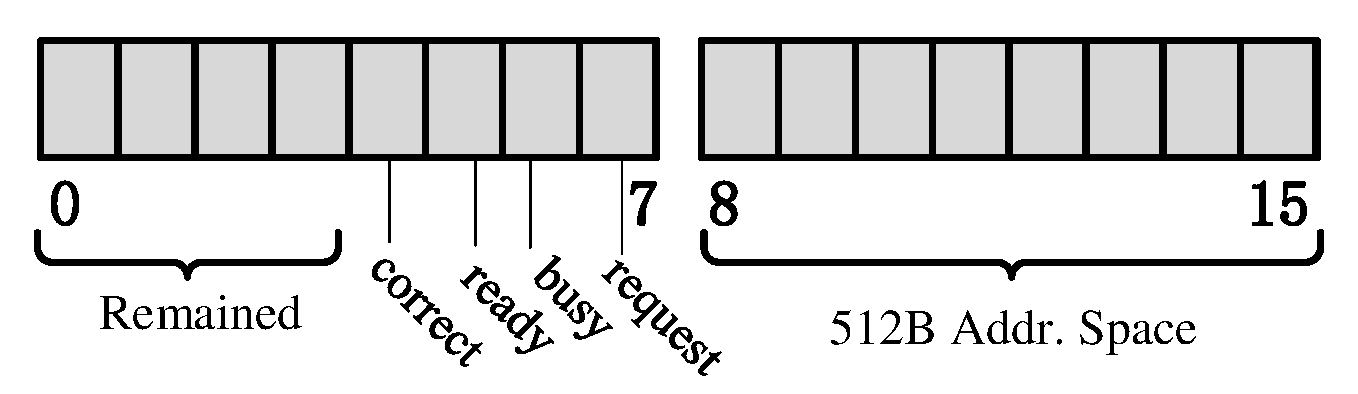
\includegraphics[width=0.4\textwidth]{VirtualDeviceAddress}
	\vspace{-5pt}
	\caption{The task completion curve of system using multiple peripherals and different capacitor sizes.}	\label{fig:CapVsBenchmark}
\end{figure}

\subsection{Explore Energy Managing Strategy Selection}
%
With an optimal hardware platform, this part explores the energy managing strategy selection with different energy supply conditions.
We scans the combination of different power traces and capacitors, and explores the suitability of different energy managing strategies.

\textbf{Three energy managing strategy candidates.\ \ }
We analysis three popular existing energy managing strategies in the energy harvesting system, that is, backup-restore~\cite{Ma2015Architecture}, state-retention~\cite{wang2017a130nm}, and DVFS~\cite{fletcher2017powerDVFS}.
\begin{itemize}

\item \textbf{State-retention}\\ 
State retention is a conventional energy managing strategy that all the peripherals enter an ultra-low cost sleep mode when the power supply is not enough.
During the sleeping stage, the system suffers a leakage power consumption to realize hardware states retention in the volatile memories.

\item \textbf{DVFS}\\ 
DVFS is an energy managing strategy used to dynamically adjust the system performance according to energy supply condition.
DVFS enables the system to execute at lower speed with lower energy consumption when the energy supply is limited, and execute at higher speed when the energy supply is sufficient.

\item \textbf{Backup-restore}\\ 
Backup-restore is a zero-leakage energy managing strategy that can bridge across power failure conditions by backing up and restoring the volatile execution states into nonvolatile memories. 
By moving the states into nonvolatile memory, the system can be safely shutdown to avoid leakage power during the outages and is most reliable in energy harvesting systems.

\end{itemize}

From the definition of the three energy managing strategies, it is obvious that, the performance of these strategies is affected by the system energy supply, which is determined the power trace and the system capacitor size.
Therefore, we explore the search space of the combination of power trace and capacitor size.
Figure~\ref{fig:HotpotGraph} (a-c) shows the performance hotpot graph when executing the \emph{brgMonitor} benchmark using each of these strategies.
% Explanations
Comparing the performance hotpot graph of these energy managing strategies, Figure~\ref{fig:HotpotGraph} (d) shows the distribution of the optimal energy managing strategy selection.
We can conclude that ...  

\begin{figure}[!htpb]
	\centering
	\vspace{-5pt}
	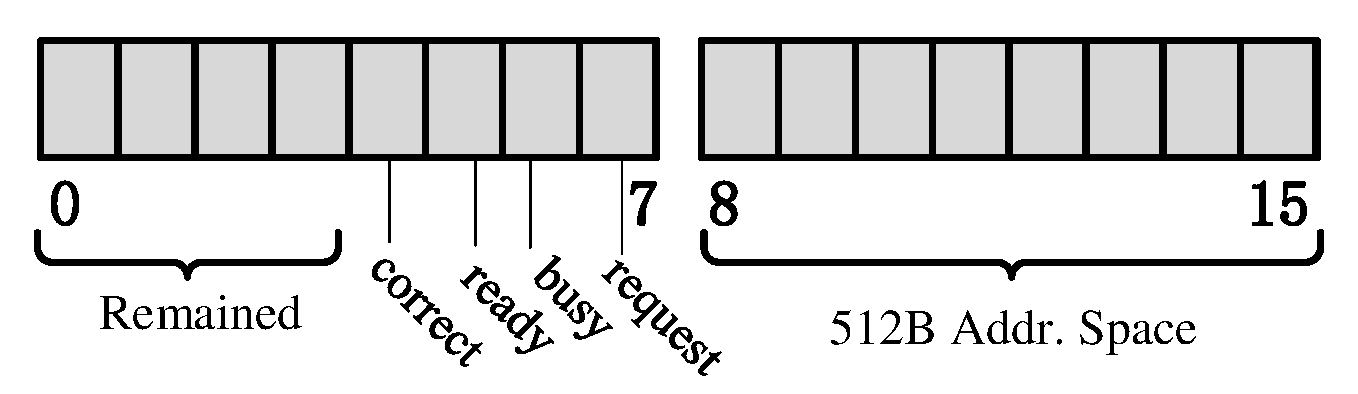
\includegraphics[width=0.4\textwidth]{VirtualDeviceAddress}
	\vspace{-5pt}
	\caption{The task completion curve of system using multiple peripherals and different capacitor sizes.}	\label{fig:HotpotGraph}
\end{figure}

\subsection{Exploration Conclusion}	\label{sec:exp-sum}
%
In conclusion, experiment explores the affect of the power supply density and the application types. 
Results show that, DVFS has the ability to take better usage of the too low and the too high energy supply.
On the other side, ModeCvrt and DVFS have the advantages in adjusting the energy usage of CPU and peripherals, respectively.
When the computing operations is dominating, DVFS has better performance to take fully usage of power supply.
When the I/O operations are dominating, ModeCvrt is the better choice to avoid the leakages of the idle peripherals.

\begin{comment}
\bibliographystyle{ACM-Reference-Format}
\bibliography{references} 
\end{comment}
\section{Conclusion}	\label{sec:sum}
%
Target on energy behavior design exploration, this paper proposes a NVP based energy harvesting system simulator, EBeSS, which supports flexible energy behavior configuration of both NVP and peripherals.
With the help of EBeSS, we explores the performance and energy efficiency of three existing energy behaviors with different power profiles and application types. 
The experiments shows the insights that both DVFS and ModeCvrt schemes have advantages in different power supply and application conditions.
Furthermore, EBeSS shows the potential to efficiently and correctly optimize the design parameter settings and validate the data consistency and correctness of the energy management strategies in the transiently powered energy harvesting systems.

\begin{comment}
\bibliographystyle{ACM-Reference-Format}
\bibliography{references} 
\end{comment}

\bibliographystyle{ACM-Reference-Format}
\bibliography{references} 

\end{document}
